\documentclass[../main/thesis.tex]{subfiles}
\begin{document}
\newpage
%% Theory

\chapter{Theory}
\label{theory}
\section{Radiation}
\label{t-radiation}
\textit{Radiation} is defined as the emission and propagation of energy through space or a material medium. Previously radiation was split into groups depending on if it was transferred through particles or waves. This was changed after 1924 when Louis de Broglie claimed that all matter has a wave-like nature. Now, \textit{particle radiation} refers to energy propagated by particles with a definite rest mass and within limits at any instant have a definite momentum and defined position. A particle beam is a group of particles that move in the same direction, similar to a light beam. Examples of these particles are electrons, neutrons, protons, and heavy ions. \textit{Electromagnetic radiation} is energy propagated  by the massless photons in phenomena such as light waves, radio waves, microwaves, X-rays, and gamma ($\gamma$) rays. Electromagnetic waves propagate at the speed of light and are represented by the spatial intensity variations of an electric field and a magnetic field. \citep[chap. 1]{Khan} 

\textit{Ionizing radiation} carries enough energy to break molecular bonds by \textit{ionizing} atoms it passes, meaning that the atom acquires a positive or negative charge. If the radiation strips an electron from the atom, it becomes a positive ion. If a stripped electron later combines with a neutral atom, it becomes a positive ion. Charged particles with enough kinetic energy is called \textit{directly ionizing radiation} because they can ionize atoms through collisions. Uncharged particles are known as \textit{indirectly ionizing radiation} as they \textit{excite} atoms, raising electrons to higher energy levels. An excited atom can later emit directly ionizing radiation through an electron. \citep[chap. 5]{Khan} See section \ref{t-int} for more on this.

%Radioactivity?

%Sources of radiation?

\subsection{Interactions of radiation with matter}
\label{t-int}
\subsubsection{Interactions of charged particles with matter}
\label{t-cp}
Charged particles, for example protons, primarily react by ionization and excitation. Electrons also commonly react through bremsstrahlung (deceleration radiation), where the particle is decelerated and emits the lost kinetic energy as a photon. When charged particles travel through a medium, they interact with atomic electrons and nuclei through the Coulomb force. These interactions can be inelastic collisions with atomic electrons, or elastic scattering without energy loss. In the inelastic collisions, the particle looses part of its kinetic energy to produce ionizations and excitations of atoms. This results in energy being absorbed in the medium as the particle is decelerated. \citep[chap. 5 $\&$ 27]{Khan} 

\textit{Stopping power} is the average rate of energy loss of a particle per unit path length ($-dE/dx$) in a medium. The \gls{let} of a particle is the energy locally deposited per length and is usually expressed in $MeV/cm$ or $keV/{\mu}m$. The \gls{let} will always be equal to or smaller than the stopping power. These parameters are used to describe energy deposition in matter and the biological effect of radiation (see section~\ref{t-bio}). The \gls{let} of a heavy charged particle (a particle of equal or greater mass than a proton) travelling through matter is inversely proportional to the square of its velocity. This means that as the particle looses energy and slows down, the rate of energy loss will increase and the particle slows down at a faster rate. The rate of energy loss (and energy deposition in the medium) becomes maximum as the particle velocity approaches zero. This leads to the particle stopping relatively quickly after travelling a certain distance and makes it possible to define a range for a certain type of particle with a defined energy in a type of matter. The intensity of a particle beam plotted versus depth in tissue can be seen in figure~\ref{fig-range} where the sudden drop in the proton plots is defined as the particle's range for that energy. \citep[chap. 27]{Khan}

\begin{figure}[h]
	\centering
	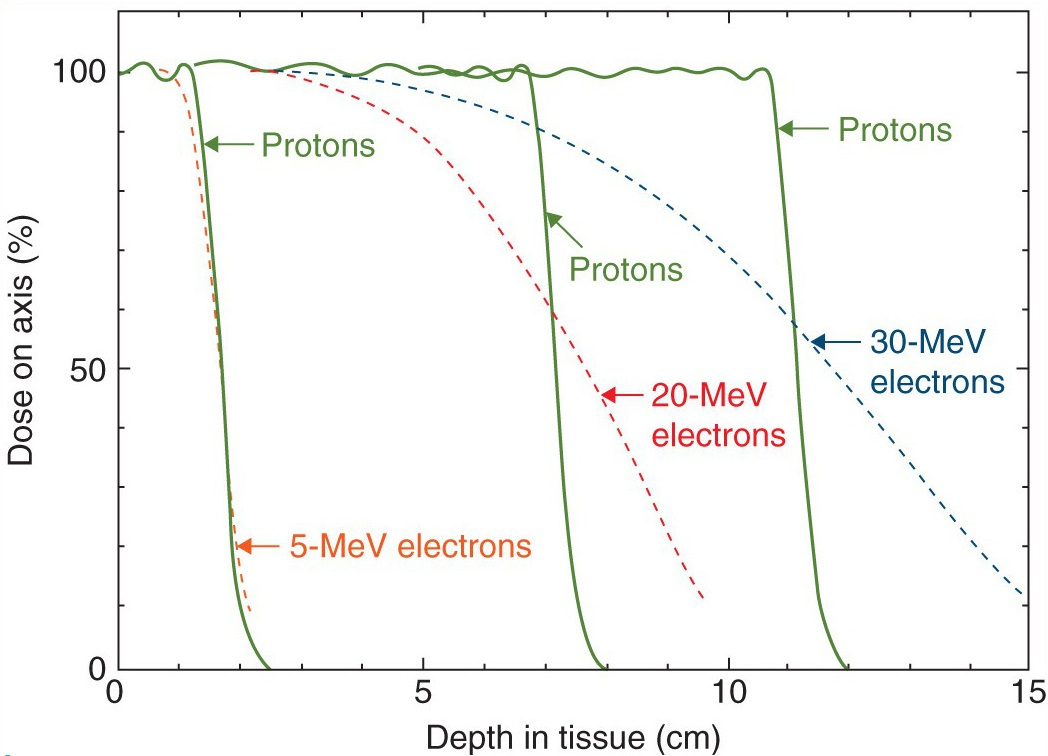
\includegraphics[width=0.8\textwidth]{figure_5_15.jpg}
	\caption{Comparison of depth dose distribution for protons and electrons of different energies. \citep[fig. 5.15]{Khan}}
	\label{fig-range}
\end{figure}

\subsubsection{Interactions of photons with matter}
\label{t-photon}
The five dominating processes for photon interactions with matter are Rayleigh scattering, the photoelectric effect, the Compton effect, pair production, and photodisintegration. Rayleigh scattering happens when a low energy photon collides with an electron and is scattered to a different angle. This does not deposit any energy in the medium, but the photon is scattered away from its original path. The photoelectric effect is a phenomenon where all the energy of a photon is absorbed in an atom. This leads to one of the orbital electrons being kicked out, and the shell vacancy will lead to emission of X-rays as a higher energy electron fills the vacancy. Occasionally, these X-rays will also kick out more electrons. The Compton effect is when a photon kicks out an electron from an atom and is scattered with reduced energy. The photons lost energy is given to the electron as kinetic energy. Pair production can happen with photons of energy greater than 1.02~MeV, where a photon travelling near an atomic nucleus gives all its energy to produce an electron and a positron. The positron will later find an atomic electron and they will annihilate each other by producing two photons of 0.51~MeV each. A high energy photon can cause photodisintegration by reacting with an atomic nucleus, leading to a nuclear reaction. \citep[chap. 2 $\&$ 5]{Khan} 

Due to all the above processes, a photon travelling through matter will at each instant in time have a certain chance of being absorbed in or scattered by the medium. Because of this, the intensity of a photon beam will start to go down instantly when it leaves vacuum, but will take a very long time to be reduced to zero, see figure~\ref{fig-photon}. It is therefore impossible to define the range of a photon beam, as is possible with a beam of heavy charged particles. The reduction in the number of photons is proportional to the number of incident photons through the \textit{attenuation coefficient}. \citep[chap. 5]{Khan} 

\begin{figure}[h]
	\centering
	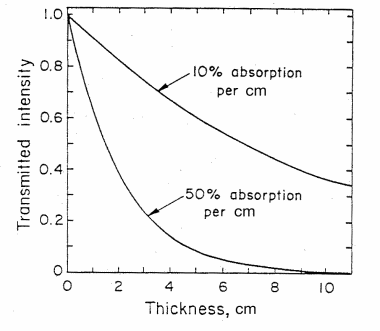
\includegraphics[width=0.6\textwidth]{asu-photon.png}%4.1?
	\caption{Photon intensity through an absorber as a function of thickness \citep{asu2000}}
	\label{fig-photon}
\end{figure}

\subsection{Biological effects of radiation}
\label{t-bio}
As discussed in the previous sections, radiation travelling through matter deposits energy in the medium. Examining the effects of this in biological tissue is an extremely complex field. Non-ionizing radiation can heat the matter it passes through, which might cause damage such as sunburns. Ionizing radiation is much more dangerous as it breaks molecular bonds, causing molecules to fall apart. This can cause massive damage to tissue cells, change the genetic material (DNA), and destroy the components that produce red blood cells. \citep[chap. 43]{UniversityPhysics} 

When a cell has been damaged by radiation, there are three possible effects: The cell dies, the cell is repaired correctly, or the cell is repaired incorrectly. The human body has very effective repair mechanisms which constantly repair cellular damage, including damage to DNA. Occasionally, these repair mechanisms will perform their function incorrectly, which can result in cells that cannot perform their normal function, or cells that damage other cells. Some of these cells are unable to reproduce themselves, while others reproduced at an uncontrolled rate, which can be the cause of cancers.\citetext{\citeauthor{jlab}}

To be able to describe the quantity of ionizing radiation for all energies, materials, and types of radiation, it is common to use the quantity \textit{absorbed dose}, or simply \textit{dose}, which is a measure of the biologically significant effects that ionizing radiation produces. It is defined as the energy delivered to tissue per unit mass. The SI unit for dose is gray (Gy), where $1 Gy = 1 J/kg$. \citep[chap. 8]{Khan} The quantity \textit{dose equivalent} has been defined because the biological effects of radiation depend on the type of radiation in addition to the dose. Dose equivalent is the dose multiplied by a quality factor for the type of radiation, in units of sievert (Sv). $1 Sv = 1 J/kg$. Additionally, the sensitivity to radiation-induced effects will vary for different types of tissue, leading to the definition of \textit{effective dose equivalent}, defined as "the sum of the weighted dose equivalents for irradiated tissues or organs". \citep[chap. 16]{Khan} 

%Dosimetry, microdosimetry?

%Vann vs tissue?
%Rekkevidde i vann?

\section{Radiation therapy}
\label{t-therapy}
Radiation therapy, also known as radiotherapy, is therapy using the biological effects of ionizing radiation to kill or control cancer cells. One of the main principles behind radiotherapy's effectiveness in treating cancer is that radiation causes much more damage to rapidly dividing cells, and tumor cells divide extremely rapidly. \citep[chap. 45]{Serway} Roughly half of all cancer patients receive radiotherapy as a part of their treatment. The radiation can originate from a machine outside the body (external beam radiation therapy), or from a radioactive source being placed into the body (internal radiation therapy). Traditional external beam radiation therapy is delivered using photon beams (photon therapy), but treatment with beams of heavy charged particles (particle therapy), like protons (proton therapy) or carbon ions, are becoming more common. Electron beam therapy is also used, mainly to treat cancer close to the surface of the body. \citep{nih}

The radiation will also damage healthy tissue, but a lot of work is put into reducing this as much as possible. Planning and simulations are done to increase the certainty of avoiding complications. Detailed imaging scans are done to get a 3D map of the patient's tumor and surrounding areas. The basis for these maps are usually \gls{CT} scans, but can also be combined with \gls{MRI}, \gls{PET}, X-ray images, or ultrasound scans. \citep{nih} One of the main reasons for \gls{CT}'s importance for photon therapy is that as it is based on photon beams, a \gls{CT} scan also yields the body's tissue-density information and photon attenuation coefficient, which is needed for photon therapy planning.  \citep[chap. 12]{Khan}

The particle beams of external beam radiation therapy are of high energy and needs to be produced in or near the treatment machine. For photon therapy, it is most common to accelerate photons using a \gls{linac}, which is small enough to fit inside the same room as the patient table. \citep{nih} For particle therapy a bigger and more expensive accelerator is needed to accelerate the particles to high enough energies. For proton therapy a cyclotron or a synchrotron is used. \citep[chap. 27]{Khan}

The dose is usually delivered once per day every workday for 4-6 weeks. One delivery is called a fraction. Fractionation is done for multiple reasons: One is to allow healthy tissue time to repair the damage from radiation. Another is to increase the chance of hitting the cancer cells at a time when they are vulnerable. Fractionation also helps to minimize the effects of random variations in the patient's position and internal geometry. \citep{fractionation} \citep{hysing-uncertain}

As already mentioned, radiation therapy also damages healthy tissue, which can produce both acute (early) and chronic (late) side effects. Acute side effects occur before the treatment ends, and is usually temporary. Examples include skin irritation, hair loss, fatigue and nausea. Chronic side effects develop months to decades after treatment is complete. Examples are skin damage, memory loss, infertility and second cancer. Second cancer is the development of a new cancer in a person that has previously had cancer. As this takes a long time to develop, it might not be a very large problem for older patients, but it is critical to avoid second cancer when treating cancer in children and adolescents. \citep{nih} 

When plotting the absorbed dose in water (or tissue), the differences between photon beams and heavy charged particle beams become even more apparent than when plotting the intensities (section \ref{t-int}). Figure \ref{fig-photonproton} shows the relative dose deposited in water for a proton and a photon beam. The photon beam's maximum is very close to the surface, and the photons will damage tissue far into the body. Also, if the tumor is deep into the body, and the beam only comes from one direction, the photons will have to do a lot of damage to the skin to be able to do enough damage to the tumor. Protons (and other heavy charged particles) on the other hand have their maximum deeper into the material, in what is called the \textit{Bragg peak}. Protons deposit less energy before the maximum, and close to no damage behind the maximum. 

\begin{figure}%[h]
	\centering
%	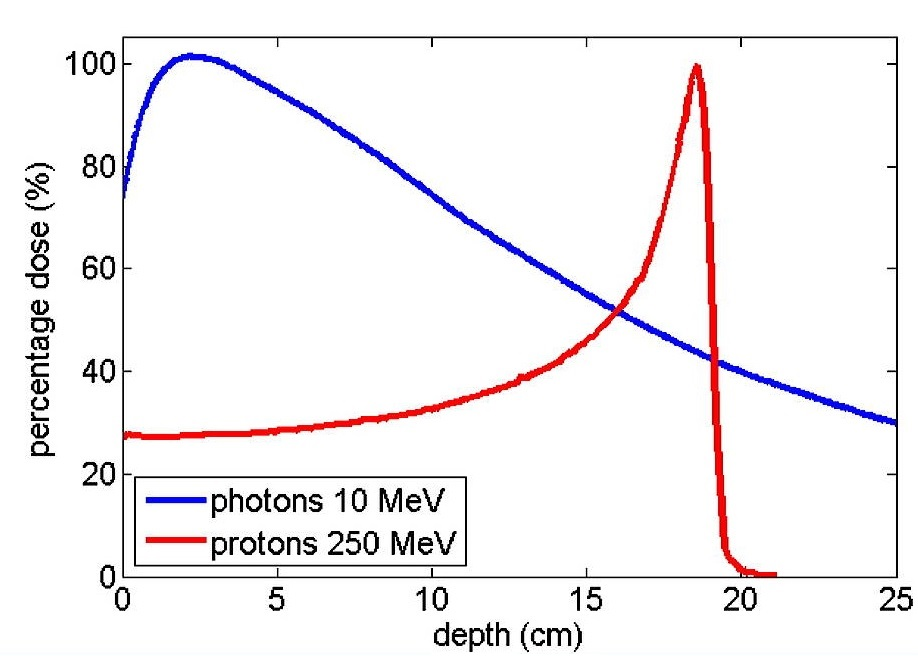
\includegraphics[width=0.7\textwidth]{swiss-photonproton.jpg}
%	\caption{Percentage depth dose for a photon beam and a proton beam in water. \citep{swiss}}
	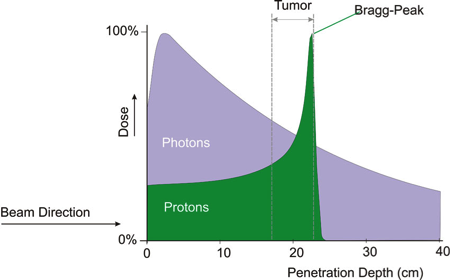
\includegraphics[width=0.7\textwidth]{pcure-photonproton.png}
	\caption{Percentage depth dose for a photon beam and a proton beam in tissue. \citetext{\citeauthor{pcure}}}
	\label{fig-photonproton}
\end{figure}

%4.18, 9.3, 27.1

\subsection{Proton therapy}
\label{t-proton}
Proton therapy is radiation therapy using high energy proton beams. The main principle behind the use of proton therapy is to exploit the Bragg peak to deposit a high dose to a tumor, with low dose delivered in front of it, and close to no dose behind. The Bragg peak is very narrow and is not able to cover most tumors, which has lead to the use of superposition of multiple beams of different energies. This superposition is called a \gls{SOBP}, see figure \ref{fig-sobp}. A \gls{SOBP} has a lot higher dose deposited in front of the tumor than a single proton beam, but it is still lower than that of a photon beam. The dose behind the tumor is still low. \citep[chap. 27]{Khan}

\begin{figure}%[h]
	\centering
	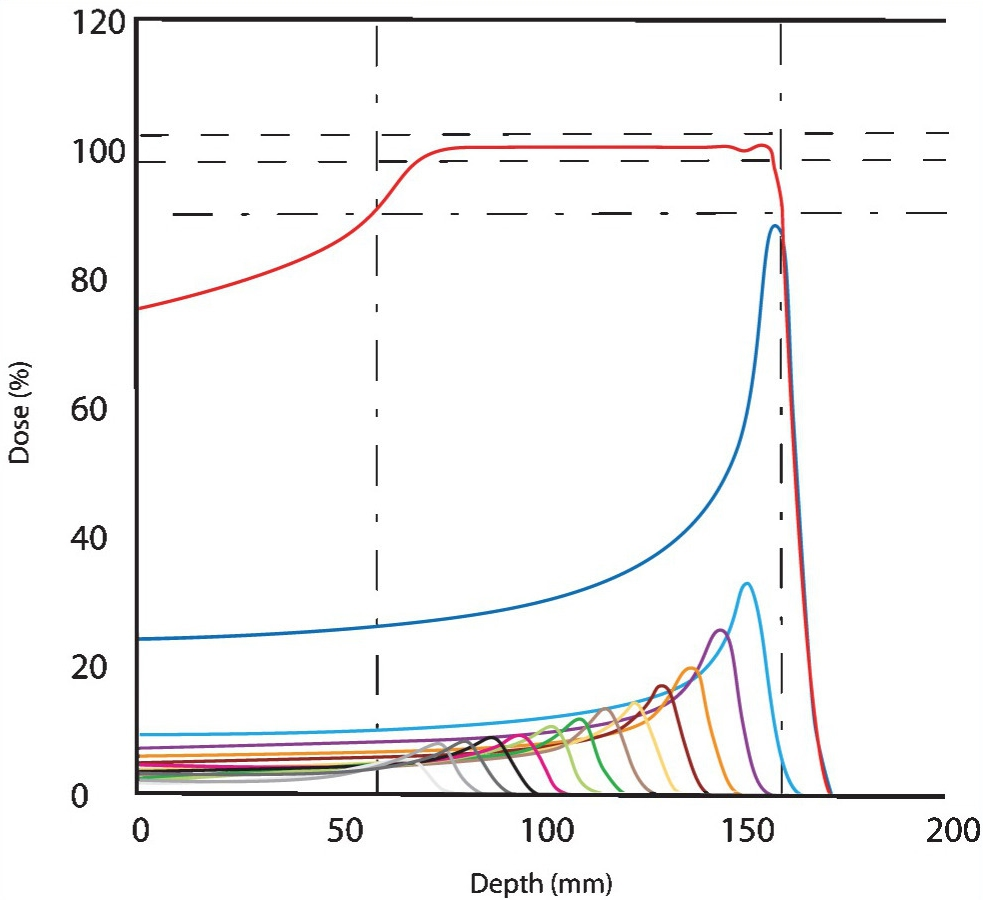
\includegraphics[width=0.6\textwidth]{figure_27_10.jpg}
	\caption{\gls{SOBP} depth dose distribution \citep[fig. 27.10]{Khan}}
	\label{fig-sobp}
\end{figure}

%Bilde av range endring? phys251 pdf

The shape of the \gls{SOBP} makes it possible to treat tumors with a lot less dose to the surrounding tissue than with photon therapy, which has two main benefits. One is the ability to treat tumors in close proximity to to critical organs without damaging said organ. The other is to avoid the chronic side effects mentioned in section \ref{t-therapy}, which is very important when treating children with cancer. \citep[chap. 27]{Khan} Figure \ref{fig-photonproton-dose} compares photon (A) and proton (B) beams, where red is high dose, blue is low dose, and gray is negligible dose. 

\begin{figure}%[h]
	\centering
	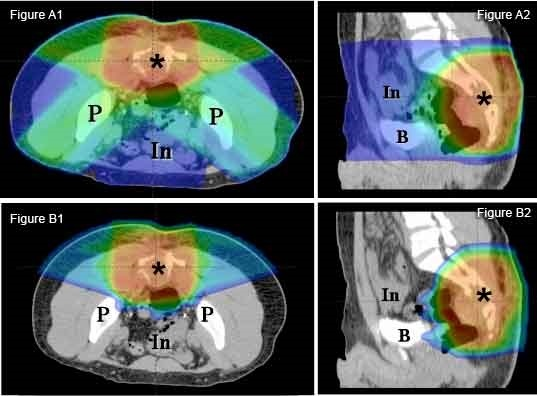
\includegraphics[width=0.8\textwidth]{pcure-dose-distribution.jpeg}
	\caption{Photon (A1 \& A2) and proton (B1 \& B2) beam dose distributions. \citetext{\citeauthor{pcure}}}
	\label{fig-photonproton-dose}
\end{figure}

The geometrical accuracy in proton therapy is a lot more critical than in photon therapy. While a geometrical error between planning and delivery in photon therapy will give a smaller under-dosage to the tumor and over-dosage to surrounding tissue, similar errors in proton therapy could cause part of the tumor receiving no dose at all and healthy tissue receiving full dose, see figure \ref{fig-miss}. Geometrical uncertainties can come from setup and anatomical variations, biological considerations, organ motion, and dose calculation approximations. \citep{Paganetti-range} 

As mentioned in section \ref{t-therapy}, photon \gls{CT} yields the patient's photon attenuation coefficient that is needed for photon therapy, but for proton therapy the stopping power is needed to greatly reduce range errors. Therefore proton \gls{CT} imaging techniques are being developed, based on the same principles as conventional \gls{CT}, but using low-intensity proton beams instead of photon beams. \citep{proton-ct}

Proton therapy can theoretically be delivered in a low fewer fraction than photon therapy due to lower dose to surrounding tissue, but this is very risky in case the target is missed.

\begin{figure}%[h]
	\centering
	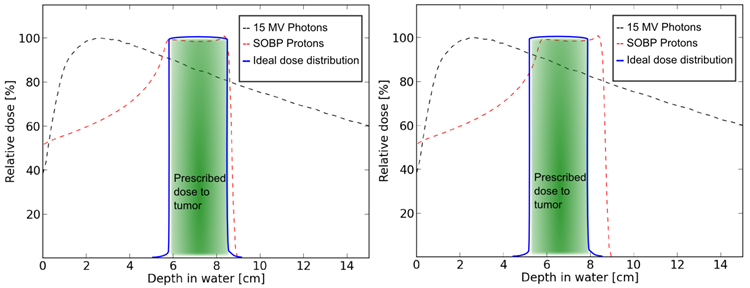
\includegraphics[width=\textwidth]{ksyh-miss.png}
	\caption{Comparison of dose distribution with correct (left) and incorrect (right) range assumptions. \citep{ksyh-phys251}}
	\label{fig-miss}
\end{figure}

\section{Radiation detectors}
\label{t-detector}
A radiation detector records interactions between incoming radiation and the detector. These interactions could be electrical, chemical, light- or heat-based. Detectors can be based on many different materials, including gas chambers, semiconductors, crystals, and liquid.\comm{\citep[chap. 9]{Thorsteinsen}} In a simple radiation detector a single particle interacts with the detector, resulting in an electric charge appearing inside the detector. This charge is typically collected by setting up an electric field inside the detector, which causes positive and negative charge to flow in opposite directions, forming an electric signal. This signal could be measured as a current (current mode), voltage (mean square voltage mode), or a charge (pulse mode). \citep[chap. 4]{Knoll}

Pulse mode is the most common readout mode because the measurement records each individual quantum of radiation. Pulse mode is therefore required when attempting to measure the energy of individual radiation events. The charge generated in the detector is usually integrated over a certain period of time. Pulse mode however does not work well at very high event rates as the time between events becomes too short to analyse the data. Current mode measures the average current over many events, therefore loosing the amplitude and timing information of individual events, but allowing for measurement with high event rates. Mean square voltage mode works much like current mode, but the output signal will be more dependent on the charge per event, making this mode more useful for mixed radiation environments. \citep[chap. 4]{Knoll}

%pulse height spectra, energy resolution, efficiency, dead time


%Dosimeter, microdosimeter?

\subsection{Semiconductor detectors}
\label{t-semi}
Semiconductor diode detectors, also called simply semiconductor detectors or solid-state detectors, are radiation detectors employing semiconductor diodes as the basic detection medium. Silicon is the most common material used, but germanium detectors are superior for gamma-ray measurements. Semiconductor detectors offer energy resolutions that are superior to other radiation detectors in addition to small size and fast timing characteristics. A big drawback is that they are degraded by radiation-induced damage during normal use. \citep[chap. 11]{Knoll}

Charged particles passing through a semiconductor detector create electron-hole pairs along the particles path. By setting up an electric potential across the diode, there will be an electric field present that will cause the holes to drift in the same direction as the electric field vector, and the electrons in the opposite direction. By monitoring one of the diodes sides, a pulse is measured as the charge from either the holes or the electrons (depending on which side is measured) is collected. 

A semiconductor detector, like other diodes, can be forward biased (positive potential on p-side) or reverse biased (positive potential on n-side). It is possible to operate a semiconductor detector without external bias, but it will perform poorly as the electric field across the junction will be too weak to read out the charge carriers before many are lost. Applying forward bias to the detector reduces the electric field even further, while reverse bias increases it. This is the main reason for reverse bias being the dominant choice for radiation detectors. \citep[chap. 11]{Knoll}

%Tran phd fig 1.3?

\subsection{3DMiMic}
\label{t-3d}
Si-3DMiMic, or simply 3DMiMic, is a silicon-based 3D mini and micro-dosimeter developed by SINTEF, which is made to mimic the response of biological tissues to ionizing radiation on a cellular and sub-cellular level. It consists of an array of 32x32 cylindrical p-i-n diodes. Each diode, or cell, is made of a 3 $\mu$m diameter n+ core cylinder, a 2 $\mu$m thick p+ trench about 10 $\mu$m further out, and a 4 $\mu$m thick n+ ring about 20 $\mu$m outside the core. The silicon between the different cells has been etched away and replaced with tissue equivalent \gls{PMMA}. %Need to double check all this later, I have contradicting sources

In the first released version of 3DMiMic, all the n+ cores in a line is connected together. Every second line is also connected, leaving two channels for readout. All the outer n+ rings are connected and can be read out if desired. 

%Need a picture


\section{Detector readout}
\label{t-read}
In different situations, the desired output from the detector readout will be different. In some cases, it is enough to simply count the radiation quanta, and in other cases one might want to read out a energy spectrum. In both cases the readout chain starts with a pre-amplifier that produces a voltage that is proportional to the radiation charge. The output from the pre-amplifier is sent to a shaping amplifier which converts the signal to a shape that is more suitable for the next component in the readout chain. This is to select the interesting pulses and convert the analog signal to a digital signal in one way or another. \citep[chap. 16]{Knoll}

\subsection{Pre-amplifier}
\label{t-amp}
For most radiation detectors, the liberated charge is too small to be processed, which is why pre-amplifiers are needed in most detector readout chains. The pre-amplifier is located close to the detector to reduce noise. A pre-amplifier can be voltage-sensitive or charge-sensitive. A voltage-sensitive pre-amplifier has an output signal proportional to the input voltage, which will be proportional to the input charge if the detector capacitance is constant. This is not the case for semiconductor detectors where the capacitance may change with the operating parameters. A \gls{CSA} has a output signal that is independent of the input capacitance as long as the amplifier gain is high enough compared to a relationship between capacitances in the system. \citep[chap. 16]{Knoll}
%fig 16.13?

One often important parameter to consider in a pre-amplifier is the dynamic range, which is the range of input signal amplitudes that can be reliably measured without changing the system. The lowest measurable input signal is limited by the noise in the system, mainly in the detector, detector cables, and pre-amplifier. A signal is not reliable if it is difficult to discern from the noise. The highest measurable input signal can be limited by the pre-amplifier or later stages, like the \gls{ADC}. If the pre-amplifier has a high gain, then a large input signal will require a higher output signal than the pre-amplifier can deliver. If the gain is low, then another stage in the system will likely be the bottleneck before the pre-amplifier reaches its highest output level. \citep{dynamic-range}

It is typically convenient to use the pre-amplifier to supply bias voltage to the detector. When this is done a single cable is used both to provide voltage to the detector and to transfer the signal pulses to the readout system. \citep[chap. 16]{Knoll}
%fig 16.16a?

\subsection{Shaper}
\label{t-shaper}
The shaper, or shaping amplifier, converts the shape of the signal to a form that is suitable for measurement. The pulse height of the signal from the shaper is proportional to the input charge. It is important that the output from the shaper quickly returns to the baseline to prevent pulse overlapping that will cause measurement errors. Tje first stage of the shaper is a differentiator (high pass filter) which passes the steep rise of the input pulse, but quickly returns to the baseline. The differentiator decides the fall time of the pulse. The signal is then amplified to a level that is suitable for the \gls{ADC}, before it is passed through the integrator (low pass filter) that filters away noise and changes the rise time of the pulse. The duration of the shaped pulse is called the shaping time. \citep[chap. 16]{Knoll}

%discriminator?

\subsection{Analog-to-Digital Conversion}
\label{t-adc}
The analog signal from the shaper needs to be converted to a digital signal for processing and storage. When it is desired to keep as much information as possible, an \gls{ADC} is used, but these use a lot of area and power. In situations where area, power, and cost is more important than accuracy of measurements (typically when there are a lot of channels), there are some simpler methods that can be used instead. The simplest is a counter, which merely counts the number of pulses with a height above a defined threshold. The information on the radiation quanta energy is lost, but the circuit is very simple. It is also possible to have multiple counters with different thresholds, which will keep some information about the distribution of radiation quanta energies. Another much used method is the \gls{ToT} technique. A \gls{ToT} circuit measures the time that the pulse is over a defined threshold, and then this measurement can be used to estimate the height of the pulse. The relationship between pulse height and \gls{ToT} is only linear within a certain range, and will usually limit the dynamic range of the readout system. \citep[chap. 6]{ToT}

%This link for ADC vs ToT: https://books.google.no/books?id=DFDRBQAAQBAJ&pg=PA173&lpg=PA173&dq=time+over+threshold+energy+measurement&source=bl&ots=J7wJ9nACVW&sig=ra60jHHnJxCc7g3g1TV2RLwHjqU&hl=en&sa=X&ved=0CBsQ6AEwADgKahUKEwi-zcfjuZTJAhUKnnIKHSQ4BAI#v=onepage&q=time%20over%20threshold%20energy%20measurement&f=false

An \gls{ADC} samples the analog signal amplitude at a certain interval (sampling rate) and converts each sampled value to a digital signal. The resolution, which is the number of bits in the digital signal, will limit the accuracy of the conversion. The quantisation error is introduced as each analog value needs to be converted to the closest digital value. The maximum percentage quantisation error can be seen in equation \ref{eq-eqmax}, where n is the number of digits in the binary code and $2^n$ is the number of digital values. \citep[chap. 10]{Bentley}

\begin{equation}%[h]
	e_q^{MAX} = \pm \frac{100}{2(2^n - 1)}\%
	\label{eq-eqmax}
\end{equation}

The dynamic range of an \gls{ADC} will mainly be limited by its resolution, noise, linearity, and jitter (small timing errors). %https://en.wikipedia.org/wiki/Analog-to-digital_converter
%Types of ADC?

\subsection{Digital Signal Processing}
\label{t-dsp}

%\subsection{Medipix}
%\label{t-medipix}

\section{Semiconductor Characterization}
\label{t-char}

\subsection{Capacitance-Voltage measurements}
\label{t-cv}
\gls{CV} profiling is a semiconductor characterisation technique that is much used to find doping- and defect densities in semiconductor junctions. The technique relies on the fact that the width of a reverse biased depletion region depends on the applied voltage. The small signal capacitance is dependent on both the doping density and width of the depletion region. \gls{CV} profiles are made by measuring the capacitance while sweeping over a voltage range. The doping density is found from the slope of a C-V curve or a $1/C^2$-V curve. \citep[chap. 2]{Schroder}

There are multiple ways to measure capacitance. A simple method is to supply a known current, and measure how fast the voltage across the capacitor rises. This method assumes an ideal capacitor, and is therefore inaccurate for a real capacitor. A more accurate method is to supply an AC signal to the \gls{DUT} and measure the AC current and voltage. A high frequency signal ($\sim$10 MHz) will be better for measuring dynamic performance, while a low frequency signal ($\sim$10 kHz) is better to find quasistatic characteristics. The capacitance is calculated from the frequency, current, and voltage. 
%https://en.wikipedia.org/wiki/Capacitance_meter
%http://www.planetanalog.com/document.asp?doc_id=527457
%Paper we got in lab

\subsection{Current-Voltage measurements}
\label{t-iv}
\gls{IV} characterization is observation of the current through a device when sweeping over the voltage across it. This can be used to find basic electrical parameters for the device. This includes leakage current, resistance, cut-in voltage, breakdown voltage, saturation voltage, and hysteresis. 

\end{document}